\documentclass[letterpaper,10pt]{extarticle}
\usepackage[utf8]{inputenc}
\usepackage[T1]{fontenc}
\usepackage{graphicx}
\usepackage{xcolor}
\usepackage{tikz}

\usepackage{amsmath,amssymb,textcomp}
\everymath{\displaystyle}

\usepackage{times}
\renewcommand\familydefault{\sfdefault}
\usepackage{tgheros}
\usepackage[defaultmono,scale=0.85]{droidmono}

\usepackage{multicol}
\setlength{\columnseprule}{0pt}
\setlength{\columnsep}{20.0pt}


\usepackage{geometry}
\geometry{left=10mm,right=10mm,top=10mm,bottom=15mm}

\linespread{1.3}


% custom title
\makeatletter
\renewcommand*{\maketitle}{%
\noindent
\begin{minipage}{0.56\textwidth}

\begin{tikzpicture}
\node[rectangle,rounded corners=6pt,inner sep=10pt,fill=blue!50!black,text width= \textwidth] {\color{white}\huge \@title};
\end{tikzpicture}
\end{minipage}
\hfill
\begin{minipage}{0.38\textwidth}
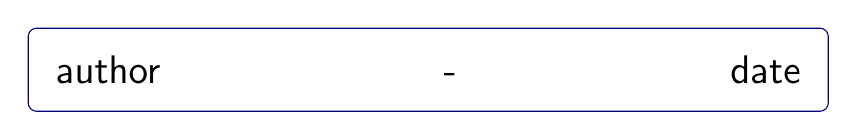
\begin{tikzpicture}
\node[rectangle,rounded corners=3pt,inner sep=10pt,draw=blue!50!black,text width= 0.78\textwidth] {\Large \@author \hfill-\hfill\@date};
\end{tikzpicture}
\end{minipage}
\bigskip\bigskip
}%
\makeatother

% custom section
\usepackage[explicit]{titlesec}
\newcommand*\sectionlabel{}
\titleformat{\section}
  {\gdef\sectionlabel{}
   \normalfont\sffamily\Large\bfseries\scshape}
  {\gdef\sectionlabel{\thesection\ }}{0pt}
  {
\noindent
\begin{tikzpicture}
\node[rectangle,rounded corners=3pt,inner sep=4pt,fill=blue!50!black,text width= 0.95\columnwidth] {\color{white}\sectionlabel#1};
\end{tikzpicture}
  }
\titlespacing*{\section}{0pt}{15pt}{10pt}

% % custom subsection
% \usepackage[explicit]{titlesec}
% \newcommand*\subsectionlabel{}
% \titleformat{\subsection}
%   {\gdef\subsectionlabel{}
%   \normalfont\sffamily\normal\bfseries\scshape}
%   {\gdef\sectionlabel{\thesection\ }}{0pt}
%   {
% \noindent
% \begin{tikzpicture}
% \node[rectangle,rounded corners=4pt,inner sep=3pt,fill=blue!50!black,text width= 0.95\columnwidth] {\color{white}\subsectionlabel#1};
% \end{tikzpicture}
%   }
% \titlespacing*{\subsection}{0pt}{15pt}{10pt}

% custom subsubsection
\usepackage[explicit]{titlesec}
\newcommand*\subsubsectionlabel{}
\titleformat{\subsubsection}
  {\gdef\subsubsectionlabel{}
   \normalfont\sffamily\small\bfseries\scshape}
  {\gdef\sectionlabel{\thesection\ }}{0pt}
  {
\noindent
\begin{tikzpicture}
\node[rectangle,rounded corners=3pt,inner sep=3pt,fill=blue!50!black,text width= 0.95\columnwidth] {\color{white}\subsubsectionlabel#1};
\end{tikzpicture}
  }
\titlespacing*{\subsubsection}{0pt}{15pt}{10pt}



% custom footer
% \usepackage{fancyhdr}
% \makeatletter
% \pagestyle{fancy}
% \fancyhead{}
% \fancyfoot[C]{\footnotesize Alexandre Francoeur - 1139118}
% \renewcommand{\headrulewidth}{0pt}
% \renewcommand{\footrulewidth}{0pt}
% \makeatother

\title{MAT265 - Équations différentielles}
\author{Examen Final}
\date{Été 2018}



\begin{document}

\maketitle

\begin{multicols*}{2}

\section{ÉD séparable}
\vspace{-2\baselineskip}
\begin{gather*}
    N(y)\frac{dy}{dx} = M(x) \quad \Rightarrow \quad N(y) \:dy = M(x) \:dx\\
    \int N(y) \:dy = \int M(x) \:dx
\end{gather*}

\section{Équations linéaires d'ordre 1}
%\vspace{-1\baselineskip}
\[y'+P(x)y=Q(x)\]
\centering
\begin{tabular}{rl}
 Étape & Formule\\
 Facteur intégrant & $\mu(x)=e^{\int P(x)dx + C}$ \\
 Solution générale & $y(x)=\frac{\int \mu (x) Q(x) dx +C}{\mu (x)}$
\end{tabular}

\section{É.D. de Bernouilli}
\[y\prime+p(x)y=q(x)y^{n}~~ | n\neq0;1 \]
\centering
\begin{tabular}{rl}
 Étape & Formule\\
 Facteur intégrant & $\mu(x)=e^{\int(1-n)P(x)dx + C}$ \\
 Variable auxiliaire & $y(x)=\frac{\int \mu(x)(1-n) Q(x) dx +C}{\mu (x)}$\\
 Solution générale & $v y^{n-1}=1$
\end{tabular}


\section{É.D. homogène}
\[\frac{dy}{dx}=f\bigg(\frac{y}{x}\bigg)\]
\centering
\begin{tabular}{rl}
 Étape & Formule\\
 Variable auxiliaire & $\int \frac{1}{f(v)-v}dv = \ln|x|+C$\\
 Solution générale & \\
 Si $v$ explicite & $y(x)=xv(x)$\\
 Si $v$ implicite & $v=\frac{y}{x}$
\end{tabular}


\section{É.D. exacte}
\[M(x,y)dx+N(x,y)dy=0\]
\raggedright
Vérification si É.D. est exacte:\\\vspace{5pt}
Si $\frac{\partial M}{\partial y}=\frac{\partial N}{\partial x}$ alors l'É.D. est exacte.
\\\vspace{5pt}
Sinon:\\\vspace{5pt}
Si $\frac{1}{N}\bigg(\frac{\partial M}{\partial y}-\frac{\partial N}{\partial x}\bigg)=f(x)$ alors $\mu(x)=e^{\int f(x)dx}$\\\vspace{5pt}
 Si $\frac{1}{M}\bigg(\frac{\partial N}{\partial x}-\frac{\partial M}{\partial y}\bigg)=g(y)$ alors $\mu(y)=e^{\int g(y)dy}$\\\vspace{5pt}
L'É.D. $\mu M dx+\mu Ndy=0 $ est une É.D. exacte.

% \frac{\partial V}{\partial x}\Leftrightarrow
% $\frac{\partial V}{\partial y}\Leftrightarrow

\[\left \{\begin{matrix} \frac{\partial V}{\partial x}=M\\\\ \frac{\partial V}{\partial y}=N \end{matrix}\right.\Leftrightarrow 
\left \{\begin{matrix} V(x,y)=\int Mdx+C_1(y)\\\\ V(x,y)=\int Ndy+C_2(x) \end{matrix}\right.\]

\section{Équations linéaires d'ordre 2}
\[Ay''+By'+Cy = f(x) \thickspace|A\neq 0\]

\subsection{Solution générale \hfill}
\[y(x)=y_C+y_P\]

\subsection{Solution complémentaire $y_C$ \hfill}
Équation caractéristique:
\[A\lambda^2+B\lambda+C=0\]
Utiliser cSolve()\\
$1^{er}$ cas:~~$b^2-4ac >0$\\

\centering
$\lambda_1$ et $\lambda_2$ deux racines réelles
\[y(x)=C_1e^{\lambda_1x}+C_2e^{\lambda_2x}\]

\raggedright
$2^{\textrm{ème}}$ cas:~~$b^2-4ac=0$\\

\centering
$\lambda=-b/2a$ racine double
\[y(x)=C_1e^{\lambda x}+C_2xe^{\lambda x}\]

\raggedright
$3^{\textrm{ème}}$ cas:~~$b^2-4ac<0$\\

\centering
$\lambda=\alpha\pm \mathbf{i} \beta$
\[y(x)=C_1e^{\alpha x}\cos(\beta x)+C_2e^{\alpha x}\sin(\beta x)\]
\end{multicols*}

%\break

\subsection{Solution particulière $y_P$}

\begin{tabular}{c|l}
$f(x)$ & Candidat à priori\\\hline
$e^{\alpha x}$ & $Ae^{\alpha x}$\\
$\cos(\omega x)$, $\sin(\omega x)$ & $A\cos(\omega x)+B\sin(\omega x)$\\
$P_{n}(x)=a_n x^n+\dots+a_1 x+a_0\thickspace|a_n\neq0$ & $A_n x^n+A_{n-1} x^{n-1}+\dots+A_1 x+A_0$\\
$e^{\alpha x}\cos(\omega x)$, $e^{\alpha x}\sin(\omega x)$ & $A e^{\alpha x}\cos(\omega x)+B e^{\alpha x}\sin(\omega x)$\\
$P_n (x)e^{\alpha x}$ & $(A_n x^n+A_{n-1} x^{n-1}+\dots+A_1 x+A_0)e^{\alpha x}$\\
$P_n \cos(\omega x)$, $P_n \sin(\omega x)$ & $(A_n x^n+A_1 x+A_0)\cos(\omega x)+(B_n x^n+B_1 x+B_0)\sin(\omega x)$
\end{tabular}

\begin{multicols*}{2}
\raggedright
{\scshape Exception:} Si le candidat à priori fait partie de $y_c$, on le multiplie par la variable indépendante autant de fois que nécessaire.



Résoudre:
\[ A\frac{d^2 y_p}{d^2 x}+B\frac{d y_p}{dx}+C y_p = f(x)\]
On trouve $A$ et $B$ et on remplace dans le candidat $y_p$




\section{Variation des paramètres}
\vspace{-2\baselineskip}
\[ y_p=C_1 (x) y_1 + C_2 (x) y_2\]
\[
W(y_1,y_2) =
\begin{vmatrix}
y_1 & y_2\\
y_1^{\prime} & y_2^{\prime}
\end{vmatrix}
=
(y_1)(y_2^{\prime}) - (y_1^{\prime})(y_2)
\]
Si $W(y_1,y_2) \neq 0$ alors:
\begin{equation*}
    y_p (x)=-y_1(x)\int \frac{y_2(x)r(x)}{W(y_1,y_2)}\:dx+y_2(x)\int\frac{y_1(x)r(x)}{W(y_1,y_2)}\:dx
\end{equation*}





\section{Mouvement rectiligne}
\vspace{-2\baselineskip}
\begin{equation*}
m\frac{dv}{dt}=\pm \:mg-kv \;\mid k>0,\;v(0)=\;\textrm{vitesse initiale}
\end{equation*}
\begin{align*}
    a(t) &= \frac{dv}{dt} = \frac{d^2x}{d^2t} = at^2 +a_0\\
    v(t) &= \frac{dx}{dt} = vt+v_0\\
    x(t) &= x_0 + v t + \frac{1}{2}a t^2
\end{align*}

\subsection{Vitesse limite théorique}
\begin{equation*}
v_\infty = \lim_{t\rightarrow 0} v(t)
\end{equation*}

\section{Circuits électriques}
\vspace{-2\baselineskip}
\subsection{Circuit RC}
\[RC\frac{dv_c}{dt}+v_c = v \;\mid v_c(0) = \textrm{tension initial du condensateur}\]

Ensuite, on trouve le courant électrique dans le circuit avec la relation:
\(i(t)=C\frac{dv_c}{dt}\)


\subsection{Circuit RL}
\[L\frac{di}{dt}+Ri=V \;\mid i(0) = \textrm{courant initial souvent}\; i(0)=0\]

\section{Loi de refroidissement Newton}
\vspace{-2\baselineskip} 
\begin{align*}
    \frac{dT}{dt} &= k(T-T_A) \\
    T &= T_A + Ce^{kt}    
\end{align*}
$T$: Température objet, $T_A$: Temp. ambiante, $k$: Constante



\section{Mélanges}
\vspace{-2\baselineskip}
\[ \frac{dq}{dt}=T_e - T_s \;\mid \textrm{où}\; T_e = \textrm{taux à l'entrée et}\; T_s = \textrm{taux à la sortie}\]


\section{Application des É.D}
\vspace{-2\baselineskip}
\subsection*{Cas particuliers}

\subsubsection{Chute libre}
\raggedright
Équation du mouvement: \(\frac{dv}{dt}+\frac{k}{m}v=g \;\mid v(0)=v_0\)\\
Avec:\\
$k$: coefficient d'amortissement
\begin{gather*}
 v\text{: vitesse} \qquad m\text{: masse} \qquad g\text{: } 9.81 m/s^2
\end{gather*}
É.D linéaire avec:
\begin{gather*}
  p(x)=\frac{k}{m} \qquad  q(x)=g
\end{gather*}
Vitesse limite: \(v_\infty = \frac{mg}{k}\)\\\vspace{2.5pt}
Vitesse instantanée: \[v(t)=v_0 e^{-\frac{k}{m}t}+\frac{mg}{k}(1-e^{-\frac{k}{m}t})\]

\subsubsection*{Circuit RL}
$V_L = L\frac{di}{dt}$\\\vspace{5pt}
$V_R=RI$\\\vspace{5pt}
Loi de kirchoff: \(V_L+V_R=V\)\\
*On suppose V constant\\\vspace{5pt}
Équation: \(\frac{di}{dt}=\frac{R}{L}i=\frac{V}{L} |i(o)=i_0\)\\
É.D de Bernouilli avec:
\begin{gather*}
 y=i \qquad p(x)=\frac{R}{L} \qquad q(x)=\frac{V}{L}
\end{gather*}
Courant limite: \(i_\infty=\frac{V}{R}\)\\
Courant instantané: \(i(t)=i_0e^{-\frac{R}{L}t}+\frac{V}{R}(1-e^{-\frac{R}{L}t})\)\\
$to=\frac{L}{R}=62.2\%$ = constante de temps\\\vspace{5pt}
$T=5e=99.3\%$ = Temps de réponse\\\vspace{5pt}

\subsubsection*{Circuit RC}
$V_R = RI = R_C\frac{dV_C}{dt}$\\\vspace{5pt}
$V_C=\frac{q}{C} = \frac{1}{C}\frac{dq}{dt}$ avec q=charge (coulombs)\\\vspace{5pt}
$i=\frac{dq}{dt}=C\frac{dV_C}{dt}$\\\vspace{5pt}
Loi de Kirchoff: $V=V_R+V_C=R_C\frac{dV_C}{dt}+V_C$\\\vspace{5pt}
Équation caractéristique: \[\frac{dV_C}{dt}+\frac{1}{R_C}V_C=\frac{V}{R_C}\;\mid V_C(0)=V_{C_{0}}\]
*avec V constant\\
\begin{gather*}
    y=V_C \qquad P(x)=\frac{1}{R_C} \qquad q(x)=\frac{V}{R_C}
\end{gather*}
$V_C$ limite: \(V_{C_{\infty}} = V\)\\
$V_C$ instantanée: \(V_C(t)=V_{C_{0}}e^{-\frac{t}{R_C}}+V(1-e^{-\frac{t}{R_C}})\)\\
On suppose que le condensateur n'était pas chargé $V_C(0)=0$\\
Tension instantannée: \(V_C(t)=V(1-e^{-\frac{t}{R_C}})\)\\
$to=RC = 63.21\%$: constante de temps\\
$T=5RC=99.3\%$: temps de réponse

\subsubsection*{Loi de refroidissement de Newton}
$T$ = température de l'objet\\
$M$ = température du milieu\\
$k$ = coefficient de proportionnalité\\
\[\frac{dT}{dt}=-k(T-M) \:\mid  k>0\]
Équation type: \[\frac{dT}{dt}+kT=kM \;\mid T(0)=t_0\]
\begin{gather*}
 y=T \qquad   p(x)=k \qquad q(t)=kM
\end{gather*}
Température limite: $t_\infty=M$\\
Température instantannée: \(T(t)=T_0e^{-kt}+M(1-e^{-kt})\)\\

\subsubsection*{Croissance logistique}
$M$ = population maximale du milieu\\
$P$ = population\\
$v$ = variation de la population\\
Équation type: \(\frac{dv}{dt}+kMv=k \;\mid v(0)=v_0\)
\begin{gather*}
 y=v \qquad    P(x)=km>0 \qquad q(x)=k
\end{gather*}
Variation limite: \(v\infty=\frac{q}{p}=\frac{k}{kM}=\frac{1}{M}\)\\
Variation instantanée: \(P(t)=\frac{P_0 M}{M e^{-kMt}+P_0 (1-e^{- k M t})}\)\\

\subsection*{Méthode générale}
\subsubsection*{Problème type}
\[\frac{dy}{dt}+Py=Q \;\mid y(0)=y_0, \;P \in\; ] 0,\infty[\;,\; Q \in\; ]-\infty,\infty[\]
É.D linéaire et séparable\\
Facteur intégrant: \(\mu(t)=e^{\int P\:dt}\)\\
Condition initiale: \(y(0)=y_0\)\\
\(y_0=\frac{q}{p}+Ce^{-pt}\)\\
\(C=y_0-\frac{q}{p}\)\\
Solution générale: \(y(t)=\frac{\int e^{pt} Q \:dt+C}{e^{pt}}\)\\
\(y(t)=y_0e^{-pt}+\frac{q}{p}e^{-pt}\)\\
Comportement à l'infini: \(y_\infty(t)=\frac{q}{p}\)\\
donc: \(y(t)=y_0e^{-pt}+y_\infty(1-e^{-pt})\)




%\pagebreak
\section{Série de Puissances}

\begin{gather*}
p(x)y^{\prime\prime} +q(x)y^{\prime}+r(x)y=0 ~~~  \left\{ \begin{array}{rcl}
y(x_0)& =& y_0\\
y^{\prime}(x_0) & = & y^{\prime}_0
\end{array} \right.
\end{gather*}

\centering
\begin{tabular}{rl}\hline
    $x_0$ & $x_0$ \\
    Points singuliers & \(p(x)=0\)\\
    Si imaginaire & \(R=\sqrt{(x_0)^2 + \beta^2}\)\\
    Sinon & \(R=x_0-\alpha\)\\
    Intervalle de convergence & \(I=]\,x_0-\beta,\; x_0+\beta\,[\)\\\hline
\end{tabular}
\\\raggedright
Solution de l'É.D.:
\begin{equation*}
    \left. y(x)=\sum^{\infty}_{n=0} a_n (x-x_0)^n  \;\;\right| x \in ]\,x_0-\beta,\; x_0+\beta\,[
\end{equation*}

\subsection{Calcul de \(a_n\) \hfill}

\subsection{Formule de récurrence \hfill}
\begin{equation*}
    \left\{ \begin{array}{ll}
        0 & n<0 \\
        a_0=y(x_0) & n=0\\
        a_1=y^{\prime}(x_0) & n=1\\
        a_n & n\geq 2
    \end{array}\right.
\end{equation*}
    

\end{multicols*}

\end{document}
